\PassOptionsToPackage{inline}{enumitem}
\documentclass[times, utf8, seminar]{fer} 
\usepackage{booktabs}
\usepackage{tikz} 
\usepackage{calc}
\usepackage{textcomp}
\usetikzlibrary{arrows,decorations.pathmorphing,backgrounds,fit,positioning,shapes.symbols,chains}
\usetikzlibrary{calc}

\usepackage{color}
\definecolor{gray}{rgb}{0.4,0.4,0.4}
\definecolor{darkblue}{rgb}{0.0,0.0,0.6}
\definecolor{cyan}{rgb}{0.0,0.6,0.6}

\usepackage{listings}
\usepackage{gb4e}

\lstset{basicstyle=\small,
columns=fullflexible,
showstringspaces=false,
commentstyle=\color{gray}\upshape,
extendedchars=true,
literate={ž}{{\v{z}}}1,
inputencoding=utf8,
upquote=true
}

\lstdefinelanguage{XML}{morestring=[b]",
  morestring=[s]{>}{<},
  morecomment=[s]{<?}{?>},
  stringstyle=\color{black},
  identifierstyle=\color{darkblue},
  keywordstyle=\color{cyan},
  morekeywords={rdfs:comment,rdf:type}% list your attributes here
}

\noautomath

\begin{document}

\title{Prikaz argumenata u informacijskim sustavima}
% 
\author{Student: Filip Boltužić}
% 
\voditelj{Prof.\ dr.\ sc. Nikola Bogunović}

\maketitle
 
\tableofcontents
 
\chapter{Uvod} 
Argumentiranje je obrazlaganje
zauzetog stajališta s ciljem uvjeravanja publike \citep{walton1990reasoning}.
Ukoliko ovaj seminar nije dovoljno dobar za položiti predmet
\emph{Predstavljanje znanja u skupovima podataka}, 
mogu se poslužiti argumentima koji će tvrditi suprotno s
ciljem uvjeravanja profesora. Pojavom interneta i 
društvenih mreža, 
argumentiranje je postalo pristupačnije no ikad; Reddit,
jedna od najvećih platformi za rasprave, 
imala je preko 1500 (234 različitih) milijuna posjetitelja
mjesečno u 2017.\ godini, koji 
diskutiraju o preko milijun različitih tematika (subreddita)
\footnote{Brojevi preuzeti 7.1.2018. s \url{https://en.wikipedia.org/wiki/Reddit} i 
\url{http://redditmetrics.com/history}}. 

Argumentacija se javlja u 
raznim oblicima: online rasprave
za ili protiv uvođenja valutne klauzule,
nadmetanje odvjetnika za pobjedu u pravnim slučajevima ili
debata oko originalnosti doprinosa znanstvenog rada.
Neke rasprave, kao online rasprave, nemaju 
strukturu ili pravila, dok 
znanstvene rasprave predstavljalju potpunu suprotnost 
s dobro definiranom strukturom rasprave (motivacija, hipoteza, 
dokaz, eksperimenti, zaključak). 
Strukturiranje rasprava olakšava ulazak novih sudionika
u raspravu, kao i kritičku analizu rasprave. Novi sudionik
strukturirane rasprave lakše će uvidjeti
i ocijeniti koji argumentima nedostaje dokaza
ili tko je počinio grešku u zaključivanju \citep{rieppel1992homology}. 
Kako izvora argumentacije ima mnogo, korištenje računala 
nameće se kao prirodan izbor za pomoć pri analizi. 
Računalna obrada argumentacije razvija se vrlo intenzivno u zadnjih 20 godina
s ciljem strukturiranja rasprava, 
donošenja novih zaključaka 
i evaluacije valjanosti argumentacije. 

% -- Sav taj online resurs predstavlja ogroman neiskoristeni izvor podataka.
% Online rasprave. Spomenuti kako su resursi nestrukturirani te kao je to jedan
% od primarnih razloga neiskorištenog potencijala argumentacijskih resursa. 
% Približiti idealnu Semantičkog weba. 

U ostatku seminarskog rada, objasnit će se pojmovi vezani uz
argument i argumentaciju (poglavlje~\ref{chap:arg}), definirati što je
računalna argumentacija i zašto je potrebna (odjeljak~\ref{chap:rac_arg}).
Nakon uvoda u računalnu argumentaciju, govorit će se o dijelovima
računalne argumentacije: 
predstavljanju argumentacije u računalu (poglavlje~\ref{chap:aif}),
analizi argumentacije (poglavlje~\ref{chap:analysis} i
evaluaciji argumentacije u računalu (poglavlje~\ref{chap:eval}).

% \section{Primjer}
% 
% -- U ovom primjeru prvo opisujemo problem koji se rješava. Ideja s ovim
% primjerom je završiti na dijagramu iz Rationalea koji onda spaja različite
% resurse i donosi zaključak
% 
% -- 2. Opisujemo okolnosti problema, koja sva znanja imamo na raspolaganju. 
% Npr. na jednoj internet raspravi su rekli X, u znanstvenom članku su otkrili
% dokaz Y, javno mnijenje ljudi na online diskusijama je Z

 %Argumentiranje i rasprave su sastavni dio naših zivota. Internetske rasprave 
 %jedan su od najzastupljenijih oblika rasprave danas. Prema istraživanju iz
 %2006. (referenca) 
 %
 %Prema istraživanju iz 2017, Reddit (jedna od najpopularnijih internetskih
 %stranica zasnovana na raspravama je 12. najposjećenija stranica u SAD-u, 25. u
 %cijelom svijetu. [referenca]. 
 %
 %Okruženje u kojem se riječ može argument pojaviti iznimno je bogato.
 %Pretraživanjem pojma argument putem najveće enciklopedije na internetu,
 %Wikipedije, moguće je dobiti sve poveznice na argument u mnogo različitih
 %domena\footnote{\url{http://en.wikipedia.org/wiki/Argument  (disambiguation)}}.
 %
 %Na današnjem webu, Web 2.0,korisnici mogu komunicirati s drugim korisnicima ili
 %web uslugama \engl{web services}, ali moguća je i interakcija između dvaju web
 %usluga. Sadržaj koji se prikazuje ograničen je dobro poznatim \emph{HTML}
 %jezikom \engl{HyperText Markup Language}. 
 %
 %Argumentima je moguće odgovoriti na pitanja: \emph{Zašto je donesena ta odluka?
 %Koje su prednosti novog zakona? Koje su mane novih mobitela?} Stoga, poznavanje
 %argumenta u korist neke teze predstavlja iznimno traženu informaciju u mnogim
 %područjima ljudskog djelovanja kao što su politika, industrija, zakonodavstvo i
 %druge. 
 %
 %Izdvajanjem argumenata iz teksta bavi se područje analiza podataka
 %\engl{information extraction}.   
 %
 %Argumenti se često referenciraju jedni na druge, pa je tako moguće jednim
 %argumentom osporiti ili ojačati drugi. Povezanost argumenata stvara podlogu za
 %stvaranje mreže argumenata grafičkim putem. Dosadašnji pokušaji strukturiranja
 %argumenta grafičkim putem rezultirali su izradom stabala argumenata.  

 
\chapter{Argument} 
Argument je skup premisa i dokaza koje podupiru neki sud. Sud je propozicija
ili tvrdnja \engl{claim} kojoj se pridjeljuje istinosna vrijednost
(\emph{istina} ili \emph{laž}). Sudovima i zaključivanjem se bavi logika.
\citep{vukovic2007matematicka}. Sudovi se donose (dodjeljuje im se istinosna
vrijednost) na temelju argumenata i procesa argumentiranja.  

Argumentiranje je verbalna i društvena aktivnost s ciljem jačanja(ili
osporavanja) diskutabilnog stajališta. Sredstvo argumentiranja su prijedlozi
ili propozicije \engl{propositions} koji opravdavaju ili opovrgavaju stajalište
nepristranom sucu s mogućnošću nepristranog racionalnog prosuđivanja
\citep{rahwan2006representing}. Argumentiranje se često proučava u sklopu
analize diskursa kao specifičan oblik razgovora \citep{palau2009argumentation}.
Prema teoriji iz \citep{van2003systematic} argumentiranje je uvijek dio
dijaloga u kojem jedna strana pokušava uvjeriti drugu u ispravnost svojih
stajališta. Dijalog ili tekst u kojem autor iznosi svoja stajališta s
pretpostavkom da očekuje protuargumente, kritike ili sumnje se smatra slobodnim
\engl{free text}. 

Teorija argumenta i argumentiranja vrlo je vjerno preslikana u pravnom sustavu.
Prilikom odlučivanja o nekom diskutabilnoj temi, suprotstavljene teme iznose
svoje argumente vezane uz temu. Iznesene argumente evaluira racionalan i
nepristran sudac te donosi odluku kojom se rješava diskutabilnost teme.
Jednostavan primjer primjene argumentiranja u sudstvu bi bio spor oko
vlasništva zemlje između susjeda. Svaki od susjeda tvrdi da mu pripada
vlasništvo nad istim posjedom. Dakle, sudovi izgledaju:

\begin{itemize} \item Susjed A tvrdi da mu pripada posjed X.  \item Susjed B
tvrdi da mu pripada posjed X.  \end{itemize}

Oba suda mogu biti podržana različtim argumentima:

\begin{itemize} \item Susjed A tvrdi da mu je posjed X pripadao u zadnjih 10
godina.  \item Susjed B tvrdi da mu je posjed X otkupio o drugog vlasnika od
susjeda A.  \end{itemize}

Ispravnost argumentata ocjenjuje sudac (ili porota) nakon čega se oba početna
suda interpretiraju (dodjeljuje im se logička vrijednost istine ili laži).  

%sada kad sam definirao što je uopće argument (vjerojatno će ići velika
%redukcija ovog napisanog), idem objasniti kako pronaći argument u tekstu s
%primjerima

\section{Definicija argumenta}

Argument može imati različite namjene. Izražavanjem \textbf{suda}, što se naziva i \textbf{izjavom} \engl{statement}, pridjeljujemo istinosnu vrijednost danoj izjavi. 
\vspace{2 mm}

\fbox{
 \addtolength{\linewidth}{-2\fboxsep}%
 \addtolength{\linewidth}{-2\fboxrule}%
 \begin{minipage}{13 cm}
  Primjer: Završio sam diplomski studij na FERu.
 \end{minipage}
} 

\vspace{2 mm}
\textbf{Uvjetni sud} \engl{conditional statement} je posebna vrsta izjave, jer razdvaja argumente na \textbf{antecedent} i \textbf{konsekvens}. Najčešće se pojavljuje kao pogodbena složena rečenica u obliku "Ako [antecedent], onda [konsekvens]".
\vspace{2 mm}

\fbox{
 \addtolength{\linewidth}{-2\fboxsep}%
 \addtolength{\linewidth}{-2\fboxrule}%
 \begin{minipage}{13 cm}
  Primjer: Ako sam završio diplomski studij na FERu, onda mogu upisati poslijediplomski studij.
 \end{minipage}
} 

\vspace{2 mm}
Čitava rečenica iz gore navedenog primjera smatra se uvjetnim sudom gdje je "Ako sam završio diplomski studij na FERu" antecedent, a "onda mogu upisati poslijediplomski studij" je konsekvens. Kao i običnom sudu, uvjetnom sudu moguće je pridjeliti istinosnu vrijednost. 

\textbf{Argument} je skup izjava, od kojih je jedna \emph{zaključak}, a ostale su \emph{premise}. Zaključak se donosi na temelju premisa.
\vspace{2 mm}

\fbox{
 \addtolength{\linewidth}{-2\fboxsep}%
 \addtolength{\linewidth}{-2\fboxrule}%
 \begin{minipage}{13 cm}
Primjer: Prema statutu je dozvoljeno upisati poslijediplomski studij samo s prosjekom ocjena višim od 3.5 tijekom diplomskog studija. Završio sam diplomski studij s prosjekom ocjena višim od 3.5, tako da bih mogao upisati poslijediplomski studij.
 \end{minipage}
}
\vspace{2 mm}

Ovdje navodnimo dvije premise, iz čega se izvodi zaključak. Argument se valorizira s obzirom na to koliko dobro premise podupiru zaključak. U ovom jednostavnom primjeru, zaključak ovisi o dvije premise koje obje podupiru zaključak. 

\section{Prepoznavanje argumenata}

Prepoznavanje argumenata u rečenici smatra se teškim problemom, i to ne samo računalna. Bogatstvo jezičnog izražaja, složeni rečenični konstrukti, implicitno zaključivanje ili uporaba ironije su samo neki od faktora koji mogu značajno otežati pronalazak argumenata u tekstu. U \citep{harrellcreating} su navedene smjernice za izdvajanje argumenata iz nestrukturiranih tekstova. Nestrukturirani tekstovi mogu biti osvrti, blogovi, odgovori na internetskim forumima, sudski zapisnici, političke zakonske rasprave \dots
U nestrukturiranim tekstovima premise i zaključci su međusobno isprepleteni, ponekad \emph{skriveni između redaka} ili povezani u istim rečenicama. 
\vspace{1 mm}

\fbox{
 \addtolength{\linewidth}{-2\fboxsep}%
 \addtolength{\linewidth}{-2\fboxrule}%
 \begin{minipage}{13 cm}
Primjer: Treba ukinuti porez na nekretnine jer neće povećati prihod u proračunu.
 \end{minipage}
}
\vspace{2 mm}

U ovom primjeru su premisa (povećanje prihoda u proračunu) i zaključak (ukidanje poreza na nekretnine) navedeni u istoj rečenici, stoga je i ovo primjer argumenta.

S obzirom na vrste riječi u rečenici argumenti se često vežu uz karakteristične uzročne i posljedične priloge, frazeme te često korištene singtagme. Svaki jezik ima svoje specifične karakteristike, stoga je identifikaciju tih ključnih riječi potrebno provesti za svaki jezik. Riječi koje upućuju da slijedi premisa mogu biti:
\begin{center}
\begin{tabular}{c c c c}
jer & zbog & iz razloga što & kako bi  \\
budući da & zato što & unatoč & pretpostavka da
\end{tabular}
\end{center}

Na isti način moguće je pronaći riječi koje se vežu uz zaključak. Identifikacijom tipičnih riječi za argumente može se olakšati posao prepoznavanja argumenata u tekstu. 
Svaki klasifikacijski zadatak često se mora znati nositi s šumovitim podacima. 
Autor teksta može iznijeti tuđi argument s kojim se ne slaže, ne navodeći razloge (premise) \engl{discount}.

\fbox{
 \addtolength{\linewidth}{-2\fboxsep}%
 \addtolength{\linewidth}{-2\fboxrule}%
 \begin{minipage}{13 cm}
Primjer: Mada poneki događaji na financijskoj burzi dionica djeluju nasumično, prema financijskim stručnjacima i njihovim dugogodišnjim istraživanjima velikih korporacija, možemo reći kako je globalno financijsko stanje stabilno. 
 \end{minipage}
}
\vspace{2 mm}

U ovom slučaju imamo glavnu premisu o istraživanju burze, koja je \emph{lažno} devalorizirana nasumičnim događajima. Moguće je ponoviti istu premisu drukčijim riječima \engl{repetition}, izraziti iznimno visoku \engl{assurance} ili nisku pouzdanost \engl{hedge} nekog događaja u obliku argumenata. 

\fbox{
 \addtolength{\linewidth}{-2\fboxsep}%
 \addtolength{\linewidth}{-2\fboxrule}%
 \begin{minipage}{13 cm}
Primjer: Očito je kako je ova generacija studenata bolja od prethodne, jer postiže mnogo bolje rezultate. No, po mom mišljenju, iduća generacija bi mogla biti još bolja.
 \end{minipage}
}
\vspace{2 mm}

Rečenične konstrukcije koje uključuju frazeme kao što su "očito je", "po mom mišljenju" i pokazuju tendencije autora prema nekom argumentu ili se koristi kako bi se čitatelju sugeriralo kako je autor lišen predrasuda. \citep{harrellcreating}. 

\textbf{Entimem} \engl{enthymeme} je argument gdje premisa i/ili zaključak nije eksplicitan \citep{bitzer1959aristotle}. Entimemi se rabe u slučajevima kada autor smatra da nije potrebno eksplicitno naglasiti zaključak.

\section{Struktura argumenata} Odnosi između argumenata mogu biti različiti. 

\vspace{1 mm}

\fbox{\addtolength{\linewidth}{-2\fboxsep}
\addtolength{\linewidth}{-2\fboxrule}
 \begin{minipage}{13 cm}
Primjer: Farmaceutska istraživanja otkrivaju nove lijekove za suzbijanje
bolesti, a zdravstvo mora biti prioritet svake državne organizacije. Dakle,
vlada bi trebala izdvajati veća sredstva za istraživanja.
 \end{minipage}
}

U ovom primjeru, razlikujemo dvije premise:
\begin{itemize}
\item farmaceutska istraživanja otkrivaju nove lijekove i 
\item zdravstvo mora biti prioritet svake državne organizacije,
\end{itemize} 
koje podupiru jedinstveni zaključak: 
\begin{itemize}
\item vlada bi trebala izdvajati veća sredstva za istraživanja.
\end{itemize}

Ovo je primjer jednog odnosa argumentiranja. Argumentiranje može biti:
\begin{itemize}
\label{itemize:naciniarg}
\item jednostavno argumentiranje (stajalište se podupire jednom tvrdnjom), 
\item višestruko argumentiranje (stajalište se podupire s višestrukim tvrdnjama) i
\item složeno argumentiranje (tvrdnje se međusobno \emph{ulančavaju}) koje može biti:
	\begin{itemize}
	\item koordinirano složeno argumentiranje (\emph{paralelno} podupiranje stajališta)
	\item podređeno složeno argumentiranje (tvrdnje se \emph{serijski} podupiru). 
	\end{itemize}
\end{itemize}

Proučavanjem dijaloga i argumenata omogućilo je strukturiranje argumenata u
grafove \citep{wolf2006coherence}. 


\subsection{Povijest mapiranja argumenata}

Analiza i prikazivanje argumenata u pravnom sustavu se nameće samo po sebi.
Prvi koji se pokušao poslužiti mapiranjem argumenata kako bi opisao pravni
slučaj bio je John H. Wigmore. Doduše, njegove metode mapiranja nikad nisu
doživile svoju praktičnu primjenu na većem broju slučaja. Richard Whately
(1859) se također bavio analizom argumenta.

Kasnije se strukturiranje argumenata počelo više koristiti u računarstvu,
točnije, obradi prirodnog jezika \citep{reed2003argumentation}. 

\subsection{Argumentacijske sheme}


Dvije najkorištenije argumentacijs



\section{Pretpostavke sustava argumentiranja} Dokazi i argumenti su dva bitno
različita pojma, pa tako izjave: \emph{P je dokaz da vrijedi T} i \emph{P je
čvrst argument u korist prihvaćanja teze T} nikako ne mogu biti smatrane
istovjetnima. Prva izjava pripada području matematička logike
\engl{mathematical reasoning}. U matematičkoj logici
\citep{bench2007argumentation}: \begin{itemize} \item ne postoje pojmovi
    nepotpune ili nesigurne informacije, \item zaključci su konačni, \item
    kontekst rasuđivanja je strogo definiran i \item sustav odlučivanja nije
    podložan raspravi te je potpuno objektivan.  \end{itemize} 

Zaključno, cilj argumenta je \textbf{uvjeravanje} \engl{to persuade}.

 
\section{Računalna argumentacija} 
\label{chap:rac_arg}
Analiza argumentacije može biti zahtjevna, kompleksna, posebice
za pojedinca. Analizom složenijih argumentacija bave se skupine ljudi,
koji za to koriste pomoć računala. 
Korištenje računala za analizu argumentacije započeo je 
\cite{dung1995acceptability}. Dung je prvi formalizirao sustav koji 
koristi oborivu \engl{defeasible} logiku zaključivanja, jer je smatrao da 
je takva logika prikladnija u argumentaciji prava i medicine
od dotad klasične logike \engl{classical logic}. Iz Dungovog rada 
nastat će \textbf{Računalna 
argumentacija} \engl{computational argumentation}, područje 
posvećeno računalnom prikazu argumentacije. 

Jedan od glavnih ciljeva računalne argumentacije je oblikovanje 
\textbf{argument weba}, velike mreže povezanih 
korisnički izraženih argumenata na Webu. Ostvarivanje argument weba 
dijeli se na \citep{Chris2017-REETAW}:
\begin{itemize}
    \item predstavljanje argumenatacije u računalu \engl{argument representation},
    \item analizu argumentacije \engl{argument analysis},
    \item podučavanje argumentacije \engl{argument pedagogy},
    \item vizualizaciju argumentacije \engl{argument navigation},
    \item evaluaciju argumentacije \engl{argument evaluation} i
    \item rudarenje argumentacije \engl{argument mining}. 
\end{itemize}




\chapter{Predstavljanje argumentacije}
\label{chap:aif}
Predstavljanje argumenata u računalima moguće kroz standardne 
serijalizacijske formate, kao što su
XML \engl{Extensible Markup Language} ili JSON \engl{JavaScript Object Notation}. 
No, radi se generičkim formatima, koji ne poznaju specifičnosti 
strukture argumenata. Nezavisno razvijeni alati kao Araucaria, Rationale 
ili Carnedeas su razvili vlastiti serijalizacijski format pohrane
argumenata. Kako je potreba za integracijom između tih alata rasla, tako
je i rasla potreba za ujedinjenim formatom pohrane argumenta. 
AIF je 2008. dobio proširenje za dijalog~\citep{reed2008aif+}.

\section{AIF}

2005. nastao je prvi prijedlog za AIF \engl{Argument
Interchange Format} jezikom \citep{chesnevar2006towards}. 
Baziran na dobro poznatom RDF jeziku, ideja AIF-a
je bila ponuditi dovoljnu ekspresivnost kojom bi se obuhvatile sve
općeprihvaćene teorije argumentacije. Začetak AIF-a se smatra prvim korakom
prema ostvarivanju Argument Web-a. 

Prije AIF-a bilo je nekoliko pokušaja stvaranja zajedničkog jezika, ponajprije
Araucarin AML \engl{Argument Markup Language}. AML, baziran na XML-u
\engl{Extensible Markup Language} osmišljen je za označavanje i analizu
argumentacije u prirodnom jeziku. Sintaksa AML jezika specificirana je pomoću
DTD \engl{Document Type Definition} strukturalnih ograničenja.  

Standardizacija definiranja računalnog jezika bila je nužna zbog tri glavna razloga:
\begin{enumerate}
    \item razmjena dokumenata kroz različite programske agente (primjerice 
korištenje dokumente kreiranog u Araucarii u Compendiumu i obratno), 
    \item kompatiblinost argumentacijskih shema u različitim programskim agentima
(primjerice, Araucaria koristi Toulminovu shemu, dok Compendium samo poznaje 
Waltonove argumentacijske sheme) te 
    \item potrebe da se automatski procesiraju logičke izjave
\end{enumerate}

\section{Specifikacija AIF-a}

AIF odlikuju 
\begin{enumerate*}
    \item sintaksa razumljiva programskim agentima,
    \item eksplicitna semantika,
    \item koncepti i proširenja 
    \item objedinjen apstraktni model koncepata i relacija između
koncepata
\end{enumerate*}

\subsection{Koncepti i relacije}

Objekti argumentacije predstavljaju se kao skup čvorova povezanih usmjerenim grafom. 
Neformalno se takav usmjereni graf u kontekstu argumentacije naziva
argumentativnom mrežom \engl{argument network} AN\@. Ne 
postoje nikakva ograničenja na oblik grafa koji može poprimiti AN.

\subsection{Čvorovi}

Razlikujemo dvije osnovne vrste čvorova: informacijske čvorove
\engl{information nodes} I-čvorove i shematske \engl{scheme nodes} S-čvorove.
I-čvorovi predstavljaju sadržaj izjava i čvrsto su povezani s temom
argumentativne rasprave, S-čvorovi predstavljaju primjenu obrazaca u
argumentiranju i smatraju se neovisnim o argumentativnoj raspravi. Postoje tri
osnovna tipa obrasca u argumentiranju: posljedica \engl{inference},
preferiranje \engl{preference} i sukob \engl{conflict}. Primjena sheme
radi se kroz S-čvor koji sukladno vrstama obrazaca u argumentiranju može biti
čvor primjene logičke posljedice \engl{inference application node} (RA-čvor), 
čvor primjene preferiranja \engl{preference application node} (PA-čvor) te
čvor primjene sukoba \engl{conflict application node} (CA-čvor).

\subsection{Bridovi}

Čvorovi su povezani usmjerenim bridovima. Kažemo da brid povezuje čvorove A i B
tako da ide iz početnog čvora A u odredišni čvor B. Razlikujemo shematske i podatkovne
bridove. Početne točke shematskih bridova su S-čvorovi, dok su početne točke 
podatkovnih bridova I-čvorovi. Primjerice, čvorovi A i B su povezani usmjerenim bridom 
$A \rightarrow B$. Ukoliko je čvor A početna točka tipa
S-čvor primjene logičke posljedice RA-čvor onda je čvor B zaključak strukture
čvora A. Čvor B može biti S-čvor ili I-čvor. Ukoliko je početni čvor I-čvor onda
odredišni čvor može biti samo S-čvor. 
Ideja iza toga stoji u principu da nije moguće povezati dvije izjave bez da se
specifira relacija (S-čvor) između izjava. 

\cite{chesnevar2006towards} navode sve moguće kombinacije S-čvorova i I-čvorova
sa bridovima uz pripadajuće semantičko značenje u tablici 1. 

\section{Primjer AIF}

% Trebam baš napraviti dijagram gdje je netko I-čvor, S-čvor...

Primjer isječka AIF dokumenta u RDF formatu vidljiv je kodu~\ref{lst:aif_rdf}.
Tip čvora definiran je kroz \textit{rdf:type} (I-čvor ili S-čvor),
\textit{aif:claimText} predstavlja sadržaj I-čvora, dok S-čvor ima različita
svojstva. U ovom primjeru imamo S-čvor zaključivanja (RA-čvor) koji nam govori
koji spaja dva čvora: \textit{aif:Premise} čvor i \textit{aif:Conclusion} čvor. 

\lstset{language=XML}
\begin{lstlisting}[caption={Primjer AIF RDF dokumenta},label={lst:aif_rdf},language=XML, captionpos=b]
<?xml version="1.0"?>
<NamedIndividual rdf:about="http://www.arg.dundee.ac.uk/AIFdb/nodes/319262">
  <rdf:type rdf:resource="http://www.arg.dundee.ac.uk/aif#I-node"/>
  <aif:claimText>Student Ivo bi trebao položiti PZUIS</aif:claimText>
  <aif:Conclusion rdf:resource="http://www.arg.dundee.ac.uk/AIFdb/nodes/319264"/>
  <aif:Conclusion rdf:resource="http://www.arg.dundee.ac.uk/AIFdb/nodes/319266"/>
  <aif:creationDate>2017-12-20 18:17:01</aif:creationDate>
</NamedIndividual>

<NamedIndividual rdf:about="http://www.arg.dundee.ac.uk/AIFdb/nodes/319264">
  <rdf:type rdf:resource="http://www.arg.dundee.ac.uk/aif#RA-node"/>
  <aif:Premise rdf:resource="http://www.arg.dundee.ac.uk/AIFdb/nodes/319263"/>
  <aif:Conclusion rdf:resource="http://www.arg.dundee.ac.uk/AIFdb/nodes/319262"/>
  <aif:creationDate>2017-12-20 18:17:02</aif:creationDate>
</NamedIndividual>

<NamedIndividual rdf:about="http://www.arg.dundee.ac.uk/AIFdb/nodes/319263">
  <rdf:type rdf:resource="http://www.arg.dundee.ac.uk/aif#I-node"/>
  <aif:claimText>Student Ivo je predao seminar</aif:claimText>
  <aif:Premise rdf:resource="http://www.arg.dundee.ac.uk/AIFdb/nodes/319264"/>
  <aif:creationDate>2017-12-20 18:17:01</aif:creationDate>
</NamedIndividual>
\end{lstlisting}


\section{AIFdb}
\label{sec:aifdb}

\begin{figure}
    \centering
    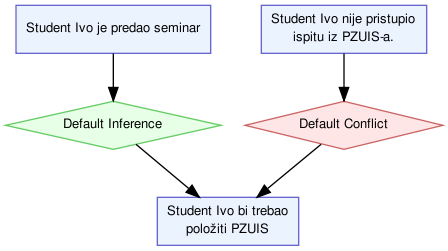
\includegraphics[scale=0.8]{aifdb_ex.png}
\caption{Primjer jednostavnog AIF dokumenta u AIFdb korisničkom sučelju}
\label{fig:aifdb_ex}
\end{figure}

AIFdb\footnote{Dostupan na \url{aifdb.org}} \citep{lawrence2012aifdb} 
je softversko rješenje za pretraživanje, pohranu i vizualizaciju AIF dokumenata te
integraciju s drugim Argument Web alatima. 
Sastoji se od tri dijela:
\begin{enumerate}
    \item korisničkog sučelja za vizualizaciju AIF dokumenata,
    \item baze podataka koja pohranjuje AIF dokumente i
    \item web servisa koji ima programski pristup bazi podataka.
\end{enumerate}
Baza podataka pohranjuje dokumente u AIF formatu tako da je 
interakcijom s bazom podataka moguće pohranjivati i pretraživati AIF dokumente. 
AIF dokumentima u bazi podataka moguće je pristupati kroz korisničko sučenje 
kroz web preglednik, ili programski, koristeći sučelje web servisa.  
U AIFdb moguće je uvesti \engl{import} dokumente u formatima alata 
Carnedeas, Rationale i Araucaria te RDF-XML formatu, te izvoziti \engl{export}
u formatima SVG \engl{support vector graphics}, DOT \engl{graph description language}
RDF te formatima alata Rationale i Carnedeas. 
Korisnik može preko web sučelja dodavati AIFdb korpuse \citep{lawrence2014aifdb}, 
koji grupiraju AIF dokumenate, i tako online pohranjivati i grupirati argumentacije. 
Jedan od korpusa dostupan online u AIFdb-u je i Araucaria korpus koji 
u trenutku pisanja sadrži 662 AIF dokumenta. 
Osim pohranjivanja, razmjene i vizualizacije AIF dokumenata, AIFdb je integriran 
s alatima Toast, Tweety i ArgSemSat koji evaluiraju arugment u AIF formatu. 
AIFdb omogućava i integraciju s OVA+ alatom tako što je moguće postojeće 
AIF dokumente modificirati kroz OVA+ alat. 
Jednostavan primjer AIF dokumenta
u AIFdb korisničkom sučelju kreiran kroz OVA+ program i 
pohranjen u AIFdb-u je na slici~\ref{fig:aifdb_ex}. Detalje poput sheme 
baze podataka moguće je pronaći u \citep{lawrence2014aifdb} i na web stranicama
centra za tehnologiju argumentacije \engl{Centre for Argument Techology} 
ARG-tech\footnote{Projekti ARG-techa dostupni na \url{http://www.arg-tech.org/index.php/projects/}}


% \begin{figure}
%     \centering
%     \def\svgscale{0.7}
%     \input{aifdb_primjer.pdf_tex}
% \end{figure}





\chapter{Analiza argumentacije}
Prvi korak u analizi argumentacije je prepoznavanje, strukturiranje i 
izrada argumenata iz argumentativne rasprave \citep{scheuer2010computer,
prudencio2005visualizing}. Izrada argumenata iz teksta
radi se izdvajajući tekst koji odgovara
specifičnim dijelovima argumenata, 
povezujući dijelove argumenta ih odgovarajućim relacijama. 
Tako u tekstu \emph{Student
Ivo polaže PZUIS;\ Student Ivo mora samo položiti PZUIS prije nego doktorira;\ Student
Ivo može doktorirati} možemo izdvojiti \textbf{premise} \emph{Student
Ivo polaže PZUIS;\ 
} i 
\emph{Student
Ivo mora položiti PZUIS prije nego doktorira
} te \textbf{zaključak}
\emph{Student Ivo može doktorirati} te izvesti da
iz premisa slijedi zaključak modus ponens pravilom zaključivanja. 
Analiza uključuje 
proučavanje valjanosti zaključivanja te
kvalitete premisa i zaključka.

Razvojem softvera za argumentaciju, 
olakšala se i analiza argumentacije. \textbf{Araucaria}
je najpopularniji softver za analizu argumentaciju s 10000 korisnika iz
preko 80 zemalja između 2001.\ i 2010.\ 
godine~\citep{Chris2017-REETAW}. Araucariom se mogu
\begin{enumerate}
\item izrađivati dijagrami argumenata iz tekstnih datoteka,
\item uređivati korištene argumentacijske modele i 
\item pohranjivati argumente (više u poglavlju~\ref{chap:aif})
\end{enumerate}
Omogućavanjem uređivanja argumentacijskih modela, Arauciaria
je prvi alat agnostičan na model argumentacije
pretpostavljajući Toulminov model argumenta, ali zadržavajući kompatibilnost
s Wigmoreovim \citep{wigmore2016wigmore} i 
Freemanovim \citep{freeman1991dialectics} modelima. 
Zbog svoje kompatibilnosti s više različitih argumentacijskih 
modela, Araucia se smatra realizacijskim začetnikom argument weba.
Araucaria je 
danas\footnote{7.1.2018.\ dostupna na URL-u \url{http://ova.arg-tech.org/}} 
dostupna online pod imenom OVA \engl{Online Visualization of Argument}. 

\section{Kolaborativna analiza}

\begin{figure}
\centering
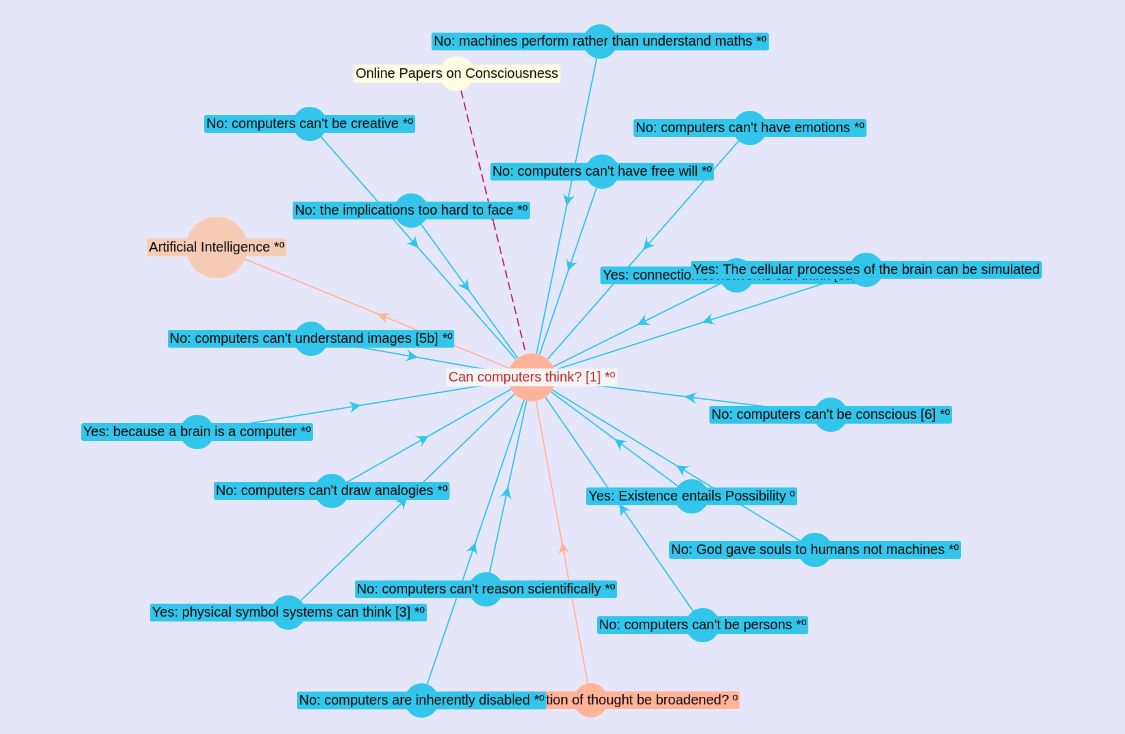
\includegraphics[scale=0.4]{debategraph.png}
\caption{Analiza mogu li računala razmišljati na DebateGraphu}
\label{fig:computers}
\end{figure}

Postavljanje sustava za analizu argumenata online olakšalo je suradnju 
na analizi argumentacije koja je neophodna u slučaju kompleksnije
argumentacije. Uz OVA alat, pojavili su se i drugi online alati za
analizu argumentacije. DebateGraph\footnote{7.1.2018.\ dostupno na 
\url{https://www.debategraph.com}} omogućava korisnicima hijerarhijsku 
analizu teme kroz grafove. Primjer na slici~\ref{fig:computers} prikazuje
analizu \emph{Mogu li računala razmišljati} u sustavu DebateGraph. Svaki
čvor u grafu moguće je dodatno otvoriti i zasebno istražiti. 

\begin{figure}
\centering
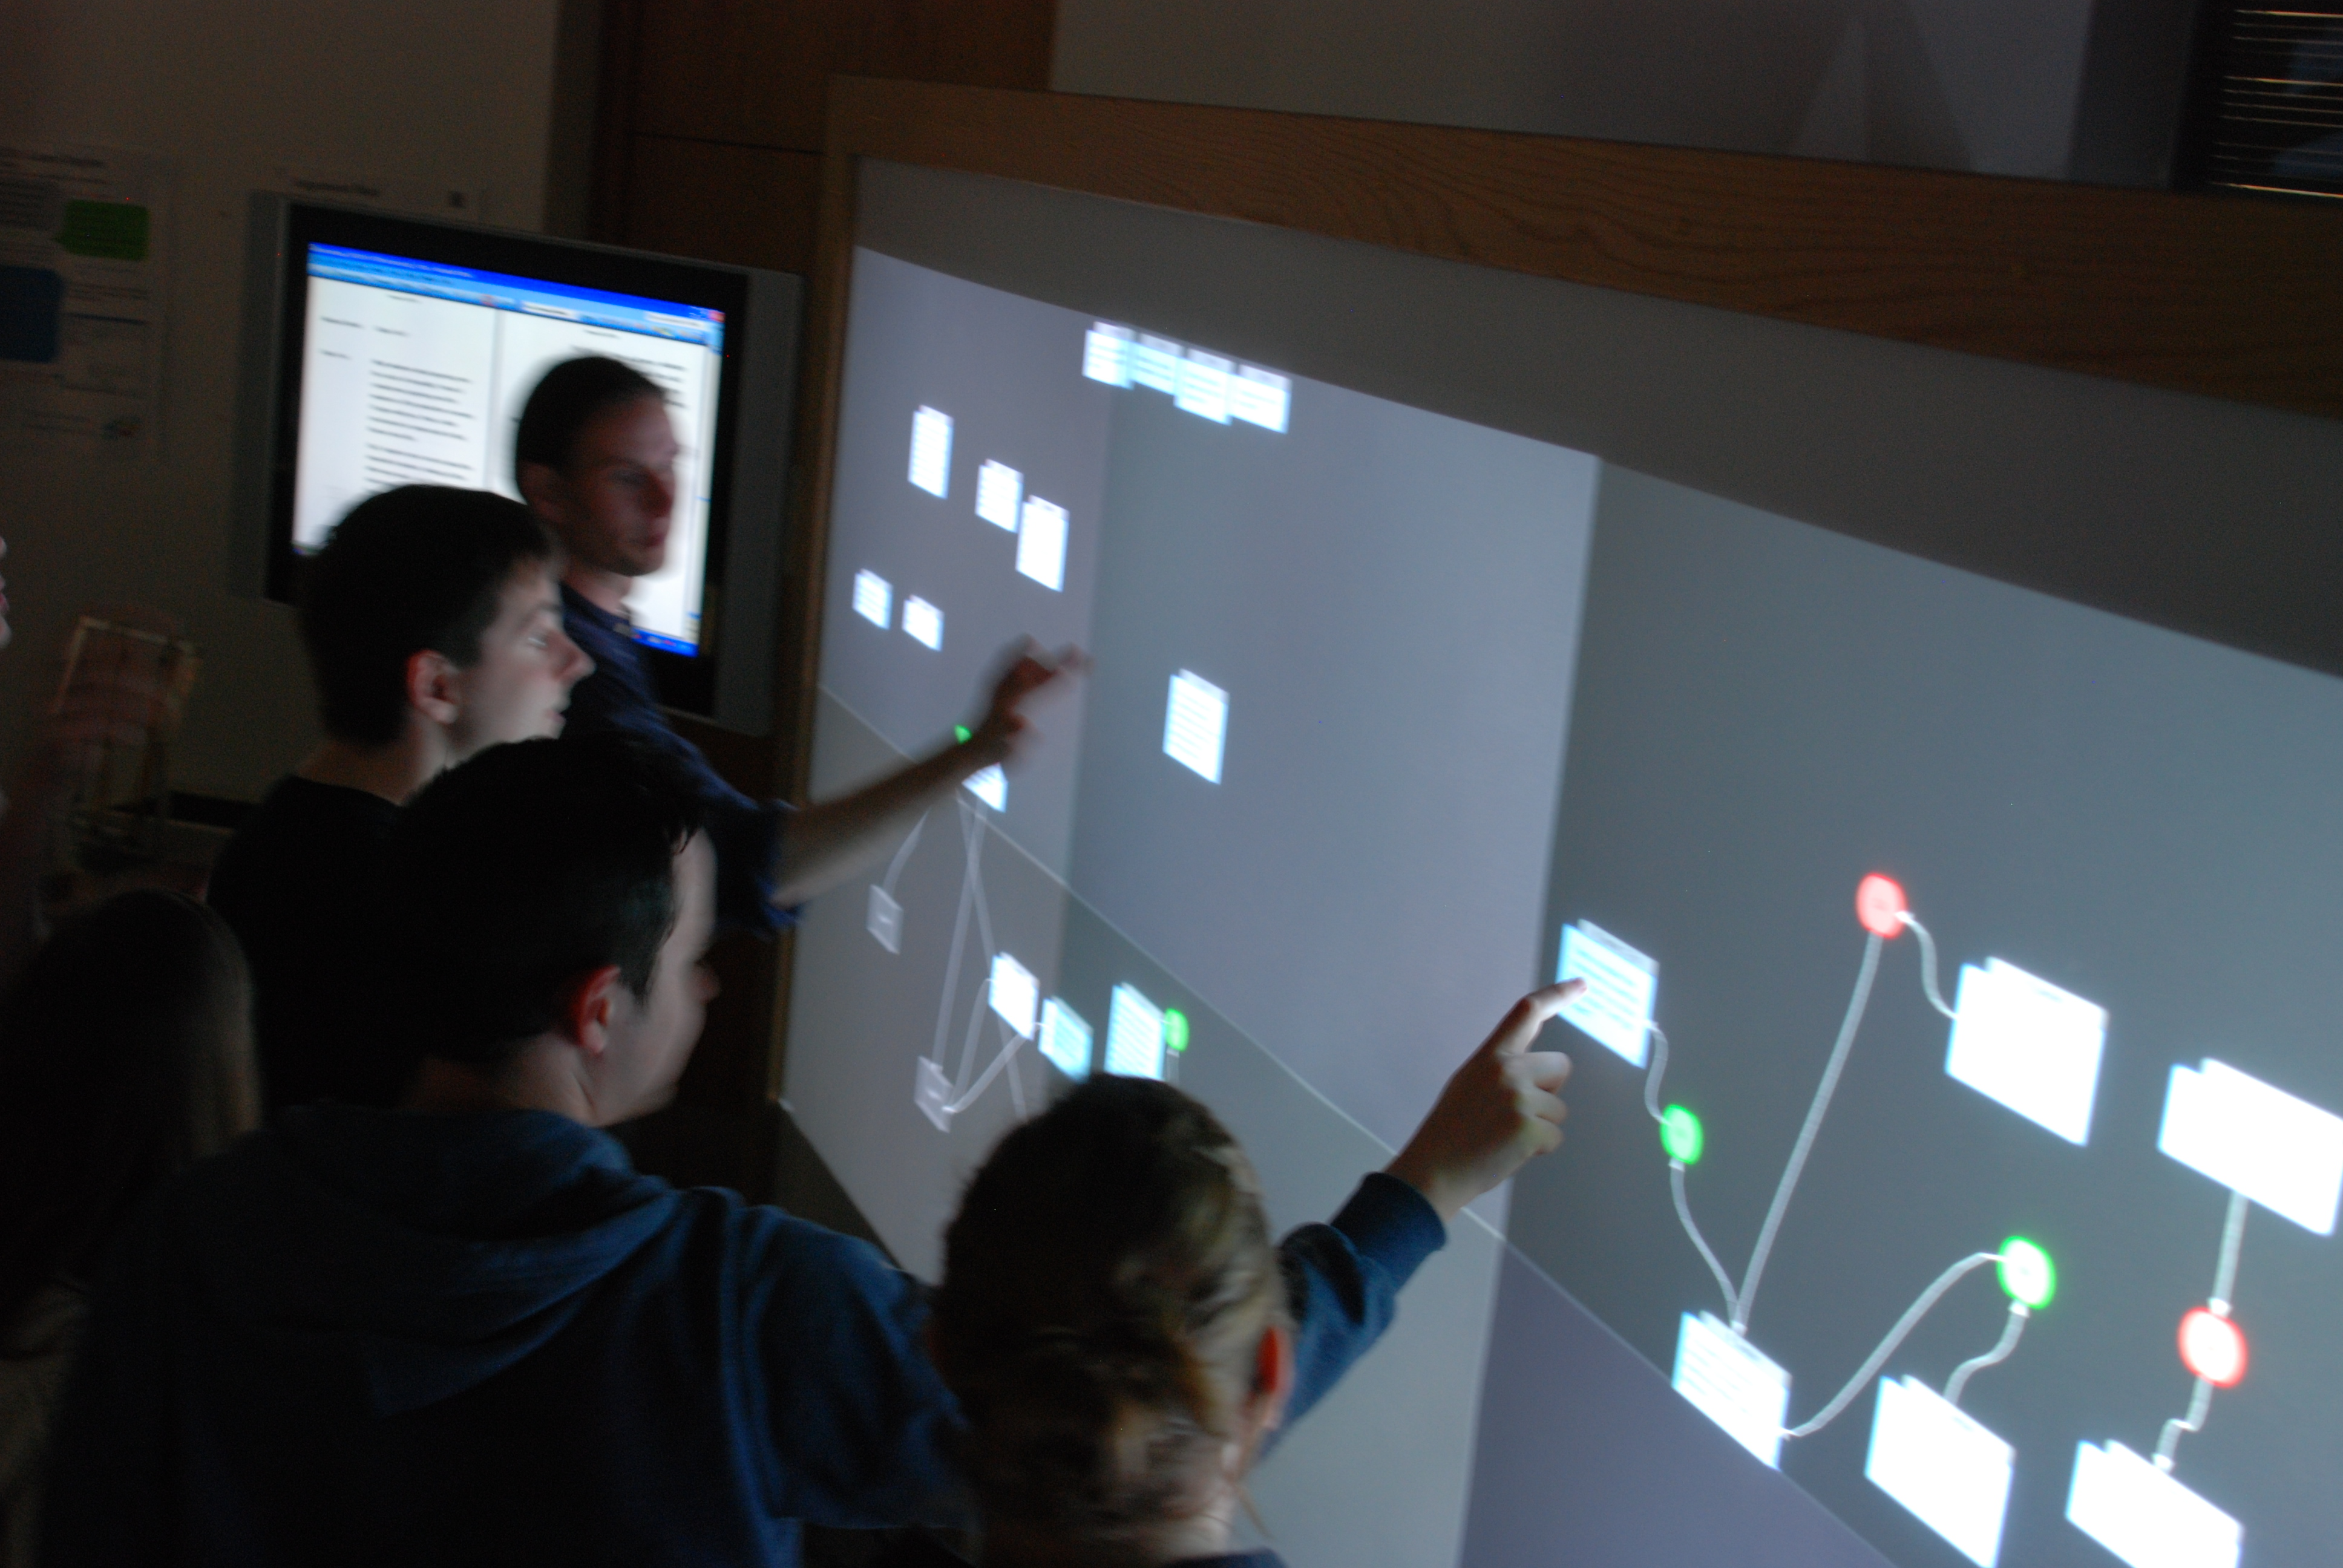
\includegraphics[scale=0.4]{analysis_wall.jpg}
\caption{Anotacija pomoću AnalysisWall-a}
\label{fig:analysiswall}
\end{figure}

Kolaborativna analiza argumentacije u stvarnom vremenu moguća je uz alat 
škotske grupe znanstvenika
AnalysisWall\footnote{7.1.2018.\ više o projektu na \url{http://www.arg-tech.org/index.php/projects/argument-analysis-wall/}}.
Uz AnalysisWall moguće je analizirati debatu, prepoznavati i povezivati argumente 
koristeći video zaslon na dodir, kao što je učinjeno na slici~\ref{fig:analysiswall}.


\chapter{Evaluacija argumentacije}
Mogućnost analize nestrukturiranih rasprava pomoću
računalnih alata uvelike pomaže stručnjacima prilikom 
vrednovanja argumentacije. No, ono što intrigira je 
mogućnost računalne evaluacije argumentacije. 
Stručnjaci obrazovani u području argumentacije znaju prepoznati
koje su prikladne logičke veze između tvrdnji.   
Stručnjaci koji se bave argumentacijom \emph{neće} reći da iz tvrdnje
\emph{Student Ivo danas nije došao na fakultet} slijedi
tvrdnja \emph{Student Ivo nije položio niti jedan predmet}.
Povezivanje argumenata logičkim vezama upravo je
razlog nastanka računalne argumentacije. 
Automatizacijom izvođenja zaključaka u argumentaciji,
moguće je doći do novih, neizrečenih tvrdnji.
Računalni sustavi za zaključivanje u argumentaciji zovu se 
\textbf{argumentacijska radna okruženja} \engl{argumentation framework}, \@{AF}.

Kao što je spomenuto u odjeljku~\ref{chap:rac_arg},
\cite{dung1995acceptability} se prvi bavio 
prihvatljivošću argumenata \engl{argument acceptability} 
kroz nededuktivnu (primjerice induktivnu ili oborivu) logiku.
Odlučio se za takvu logiku jer je primjetio da se ljudi u svakodnevnom 
govoru ne služe izjavama prikladnima za zaključivanje u formalnoj logici. 
Tako se ljudi u svakodnevnom govoru služe analogijama i induktivnom zaključivanju, 
primjerice: izjava \emph{Student Ivo je položio skoro sve predmete na doktorskom studiju} 
ima za logičku posljedicu \emph{Student Ivo će položiti PZUIS, predmet na doktorskom studiju}. 
Dakako, ova izjava nije valjana prema formalnoj logici, oblikovana je
induktivnim argumentom analogije koji se često koristi u svakodnevnom govoru 
\citep{juthe2005argument}.

U sklopu razvoja argument web-a, razvijeno je nekoliko sustava za
automatsku evaluaciju argumentacije, kao i argumentativnih radnih okruženja
zasnovanih na Dungovoj ideji. Najkorištenije argumentacijsko radno okruženje
je \textbf{ASPIC+} okruženje. 
Prvi računalni sustav, implementacija argumentacijskog radnog okruženja, 
je \emph{Dung-O-Matic} \citep{snaith2010pipelining},
no taj sustav nije kompatibilan s ostalim formatima zapisa argumenta. 
\emph{TOAST} sustav razvijen je s funkcionalnostima Dung-O-Matic-a, ali 
je kompatibilan s popularnim AIF formatom (poglavlje~\ref{chap:aif}), kao i sa 
ASPIC+ argumentacijskim radnim okruženjem. 
Postoje još brojni drugi sustavi kao što su Tweety \citep{thimm2014tweety} koji
pokušava mapirati AIF strukturu u logički program 
(slično kao i ASPARTIX \citep{egly2008aspartix}),
ArgSemSAT \citep{cerutti2014argsemsat}
koji koristi poznatu SAT \citep{moskewicz2001chaff}
 tehniku kako bi odredio prihvatljivost argumenta
u argumentacijskom radnom okruženju.

\section{ASPIC+}
\label{sec:aspic}

$AF$ je par $(A, D)$ gdje je $D \subseteq A \times A$ binarna relacija napada između argumenata $A$. 
Kažemo da $A$ napada $B$ ukoliko $A$ napada $B$ i $B$ ne napada $A$. $A$ 
predstavlja skupove argumenata, proširenja \engl{extensions}
koji su koherentni i brane se od napada. 
Za svaki $X \in A$, $X$ je prihvatljiv s obzirom na $S \subseteq A$ akko
$\forall Y$ takav da $(Y, X) \in C$ implicira $\exists Z \in S$ takav da
$(Z, Y) \in D$. Ako je $S \subseteq A$ bez konflikta \engl{conflict free}, što znači 
da ne postoje $A \in S, B \in S$ takvi da postoji $(A, B) \in D$ onda:
\begin{itemize}
    \item S je \emph{prihvatljivo} proširenje akko $X \in S$ implicira prihvatljiv $X$ prema $S$;
    \item S je \emph{kompletno} proširenje akko $X \in S$ akko je $X$ prihvatljiv prema $S$;
    \item S je \emph{preferirano} proširenje akko je uvrštenje skupa maksimalno potpuno proširenje; 
    \item S je \emph{osnovno} proširenje akko je uvrštenje skupa minimalno potpuno proširenje; i
    \item S je \emph{stabilno} proširenje akko je preferirano i $\forall Y \notin S, \exists X \in S$ takav da
        $(X, Y) \in D$
\end{itemize}
Za $T \in $\{kompletan, preferiran, osnovan, stabilan\}, $X$ je
\emph{skeptično} opravdan ukoliko $X$ pripada barem jednom $T$ proširenju
\citep{modgil2014aspic+}. 

Za korištenje ASPIC+-a potrebno je odabrati negacijsko-zatvoreni logički jezik $L$,
dva skupa strogih \engl{strict} i oborivih \engl{defeasible} pravila
zaključivanja. 
Osim pravila, potrebno je specifirati bazu znanju 
\engl{knowledge base} koja sadrži dostupne informacije u obliku premisa. 
U bazi znanja razlikujemo obične, aksiome, te oborive premise, koje je moguće
napadati. Baza znanja, pravila zaključivanja i logičkog jezika
zajedno čine \textbf{argumentacijsku teoriju} \engl{argumentation theory}.
ASPIC+ radi nad argumentacijskom teorijom i omogućava upite nad njom. 
Nad zadanim argumentom moguće je dobiti premise koje ga čine kroz
upit $Prem$, zaključak upitom $Conc$, 
njegove podargumente upitom $Sub$, oboriva pravila argumenta upitom $DefRules$ te
zadnje pravilo zaključivanja upitom $TopRule$. 

\begin{figure}
    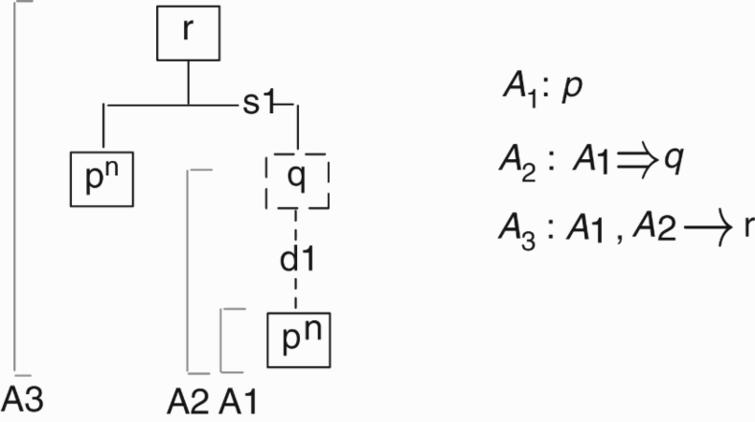
\includegraphics[scale=0.6]{aspic.jpg}
    \caption{Primjer argumenta u ASPIC+ sustavu}
\label{fig:aspic}
\end{figure}

Primjerice, baza podataka se sadrži od:
$p, q, r, s, t, u, v, w, x, d_1, d_2, d_3, d_4, d_5, d_6$ i njihovih negacija, gdje 
je skup strogih pravila $R_s = \{s_1, s_2\}$, a skup oborivih pravila
$R_d = \{d_1, d_2, d_3, d_4, d_5, d_6\}$. Sama pravila su:
\begin{align*}
    d_1&: p \Rightarrow q  &   d_4&: u \Rightarrow v   &    s_1&: p, q \rightarrow r \\
    d_2&: s \Rightarrow t  &   d_5&: v, x \Rightarrow \neg t  &    s_2&: v \rightarrow \neg s \\
    d_3&: t \Rightarrow \neg d_1  &  & d_6 s \Rightarrow \neg p
\end{align*}
Funkcija $n$ pridjeljuje oborivom pravilu $d_i$ formulu $d_i$, dakle vrijedi:
$n(d_i) = d_i$, prikazano na primjeru: $n(p \Rightarrow q) = d_1$. Ovako definiran argument
prikazan je slikom~\ref{fig:aspic}: premise su na dnu slike, a zaključak na vrhu. Premise
su označene eksponentom, a oborive premise i zaključivanja isprekidanom linijom. 
Sada je i upitima moguće doći do elemenata argumenata $A_1, A_2$ i $A_3$. Tako je
$Prem(A_3) = \{p\}$, $DefRules(A_3) = \{d_1\}$. Još primjera i pojašnjenja ASPIC+
radne okoline moguće je pronaći u \citep{modgil2014aspic+}. 

\section{TOAST}

TOAST \engl{The Online Argument Structures Tool} je implementacija ASPIC+ 
\citep{modgil2014aspic+} argumentacijskog okruženja. TOAST je web servis 
u koji je moguće unijeti argumente i evaluirati ih. 
Korisnik TOAST-a može unositi izjave u bazu znanja \engl{knowledge base}
i definirati vlastita pravila \engl{rules} (prema ASPIC+-u). U bazi znanja 
razlikujemo aksiome, premise i pretpostavke. Osim standardnih logičkih
poveznica koje je moguće unositi između tvrdnji u bazi znanja, 
između premisa i pretpostavki moguće je definirati relacije preferencije. 
Pravila se unose u formatu:
\lstset{language=XML}
\begin{lstlisting}[caption={},label={lst:format},language=XML, captionpos=b]
[jedinstvena oznaka] {lista ancedensa}{implikacija}{konsekvens};
\end{lstlisting}
primjerice pravilo s dvije tvrdnje iz kojih logičkom implikacijom slijedi konsekvens:
\lstset{language=XML}
\begin{lstlisting}[caption={},label={lst:format},language=XML, captionpos=b]
[p] {Student Ivo studira na FER-u, FER je u Zagrebu}{->}{Student Ivo studira u Zagrebu};
\end{lstlisting}
Osim relacija klasične logike, moguće je preferirati tvrdnje (PA-čvor) u formatu:
\lstset{language=XML}
\begin{lstlisting}[caption={},label={lst:format},language=XML, captionpos=b]
    [jedinstvena oznaka pravila a] < [jedinstvena oznaka preferiranog pravila b] 
\end{lstlisting}
Primjeri korištenja TOAST-a vidljivi su na slikama~\ref{fig:toast_in} i~\ref{fig:toast}.
TOAST je u potpunosti integriran s AIFdb (više u odjeljku~\ref{sec:aifdb}), stoga je 
moguće argument kreiran u AIFdb-u evaluirati kroz TOAST.\@

\begin{figure}
    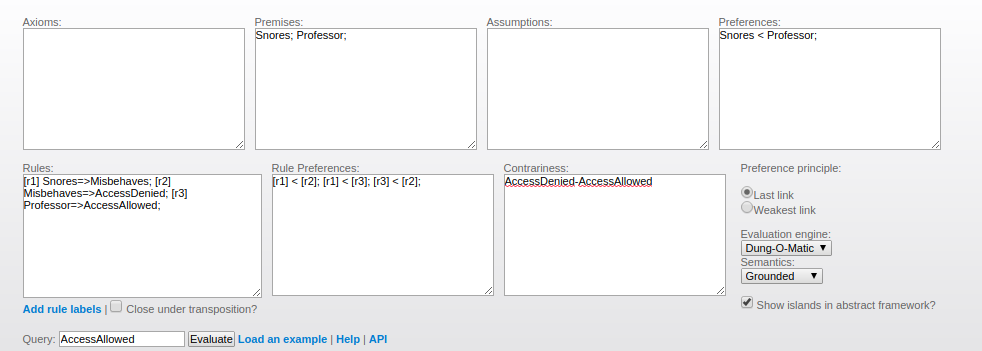
\includegraphics[scale=0.4]{toast_input.png}
    \caption{Unos pravila i baze znanja u TOAST}
\label{fig:toast_in}
\end{figure}

\begin{figure}
    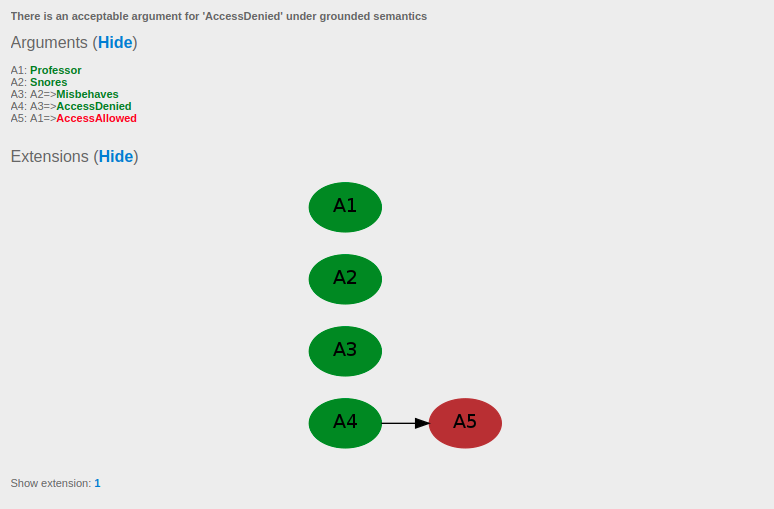
\includegraphics[scale=0.4]{toast.png}
    \caption{Evaluacija prihvatljivosti \emph{AccessDenied} upita}
\label{fig:toast}
\end{figure}


\chapter{Zaključak} Zaključak.

Zakljucak. 

\bibliography{literatura} \bibliographystyle{fer}

\chapter{Sažetak} Sažetak.

\end{document}
